\chapter{Conclusion}
\thispagestyle{empty}
\section{Summary}

This capstone project offers a valuable opportunity to delve into essential areas of mathematics, showcasing the elegance of logical reasoning in this field and its applicability to machine learning. Our study builds progressively across several branches, including real analysis, measure theory, probability and stochastic processes, and ultimately, stochastic differential equations (SDEs). We have compiled the necessary theorems for the reverse-time equation, the foundational element for diffusion models using SDEs. Additionally, we have thoroughly explored the Transformer neural network architecture, focusing on its Positional Embedding and Attention Mechanisms.

On the practical side, we conducted experiments with various segmentation and inpainting models to identify the most effective methods for watermark removal. Throughout this process, we addressed and resolved technical challenges related to performance and memory, enhancing our engineering skills in the field of Artificial Intelligence. The result is a comprehensive pipeline that processes a watermarked image and outputs an unwatermarked version while preserving the original structure of the image. Additionally, our pipeline outperforms some methods when using the two-stage pipeline, which involves localizing the watermark first and then removing it, making it possible to improve sub-task models. Furthermore, we experimented with and achieved noticeable results on a Zero-shot pipeline, making our model flexible to use on any dataset.



\section{Limitations and Future Work}
\subsection{Limitation}
% \subsubsection{Processing Time}

% \subsubsection{Processing Time}

In our pipeline, it takes about 1.5-2.5 seconds to complete one inference, which is quite time-consuming and may require users to wait if they want to remove watermarks from multiple images. Additionally, our problem is limited to visible watermarks and focuses on processing images, without deep exploration and development on other types of watermarks. Furthermore, our watermark dataset is small, as it only covers Pokemon-themed watermarks and lacks generalization to all visible watermarks. For the zero-shot methods we implemented in this report, they still require detailed instructions from users, such as points or boxes, and have not been tested on more natural instructions like language or simply a text sentence. We will continue to research and improve our limitations in the future. 


\subsection{Future Work}
In the future work, we will develop Zero-shot methods using text prompts. We find this to be entirely feasible as we experimented with a model that allows us to align images and text, namely CLIP \cite{radford2021learning}. This model is trained on hundreds of thousands of image-text pairs with the aim of learning mutual features and can be used as a feature extraction layer, where the text prompt provides the class that the image is associated with, allowing the model to generate attention heatmaps on the image, highlighting objects related to the prompted text. The results of our experiments with the pretrained CLIP model on watermark data are shown in Figures \ref{fig:pic_of_pokemon} and \ref{fig:pic_of_wtm}.

In Figures \ref{fig:pic_of_pokemon} and \ref{fig:pic_of_wtm}, we can see that when prompted with "Pokemon," the model immediately focuses on the Pokémon in the center of the image, and when prompted with "Watermark," the model provides some points that are likely watermarks. By using CLIP in this way, we can leverage it to extract features from text prompts and make accurate predictions as needed.
\begin{figure}[t]
    \centering
    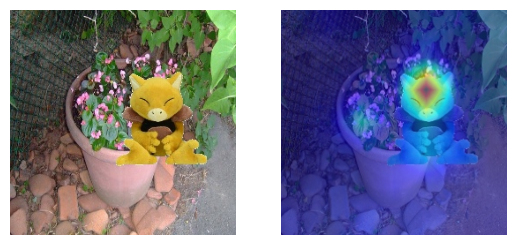
\includegraphics[width=0.75\linewidth]{img/pic_of_pokemon.png}
    \caption{CLIP attention heatmap with text prompt \textit{The picture have pokemon}}
    \label{fig:pic_of_pokemon}
\end{figure}

\begin{figure}[t]
    \centering
    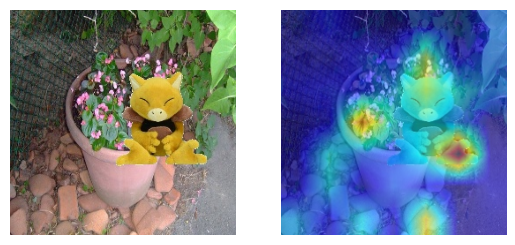
\includegraphics[width=0.75\linewidth]{img/pic_of_wtm.png}
    \caption{CLIP attention heatmap with text prompt \textit{The picture have watermark}}
    \label{fig:pic_of_wtm}
\end{figure}

\begin{figure}[t]
    \centering
    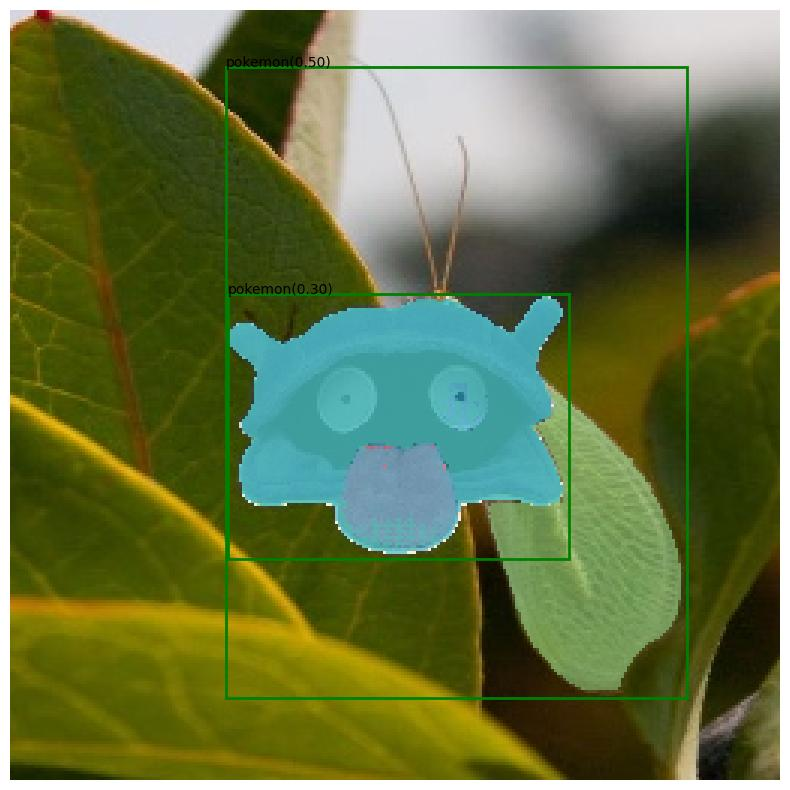
\includegraphics[width=0.75\linewidth]{img/groundedsam.png}
    \caption[Zero-shot text prompt result with Object Detection and SAM box prompt]{Zero-shot text prompt \textit{The picture have pokemon} result with Object Detection and SAM box prompt}
    \label{fig:groundedsam}
\end{figure}
Furthermore, in our experiments with SAM, we found that using bounding boxes as input for SAM is entirely promising. We have researched and are developing a model related to Zero-shot object detection using text prompts. The trial results of our team are shown in Figure \ref{fig:groundedsam}. Specifically, in this image, we also used the prompt "\textit{The picture has pokemon}" to indicate that there are Pokémon in this image, even though the model has never learned about Pokémon before. Nonetheless, it still makes predictions of two potential bounding boxes. From there, the team used these bounding boxes as input for SAM and found that it was able to detect and segment them. However, due to the limited time of the thesis and the results not meeting expectations, the team decided to continue researching this aspect for the next phase.